\documentclass[twocolumn,twocolappendix,trackchanges]{aastex63}
\usepackage{amsmath}
\newcommand{\code}[1]{\texttt{#1}}
\newcommand{\mesa}{\code{MESA}}
\newcommand{\MESA}{\code{MESA}}
\renewcommand{\labelitemii}{$\bullet$}
\newcommand{\kms}{{\mathrm{km\ s^{-1}}}}
\newcommand{\Msun}{{\mathrm{M}_\odot}}
\newcommand{\kev}{\mathrm{keV}}
\newcommand{\gk}{\ensuremath{\,\rm{GK}}}
\usepackage{CJK}
\DeclareRobustCommand{\Eqref}[1]{Eq.~\ref{#1}}
\DeclareRobustCommand{\Figref}[1]{Fig.~\ref{#1}}
\DeclareRobustCommand{\Tabref}[1]{Tab.~\ref{#1}}
\DeclareRobustCommand{\Secref}[1]{Sec.~\ref{#1}}
\newcommand{\zoph}{$\zeta$ Oph}

\newcommand{\todo}[1]{{\large $\blacksquare$~\textbf{\color{red}[#1]}}~$\blacksquare$}

\defcitealias{villamariz:05}{VH05}


\begin{document}

\graphicspath{{./figures/}}


\title{Testing models of accreting stars in
  massive binaries on $\zeta$ Ophiuchi}
\author[0000-0002-6718-9472]{M.~Renzo}
\affiliation{Department of Physics, Columbia University, New York, NY 10027, USA}
\affiliation{Center for Computational Astrophysics, Flatiron Institute, New York, NY 10010, USA}

\author{Y.~G\"otberg}
\affiliation{The Observatories of the Carnegie Institution for Science, 813 Santa Barbara Street, Pasadena, CA 91101, USA}


\begin{abstract}
  Binarity dominates the evolution of massive stars, and the nearest
  O-type star to Earth, $\zeta$ Ophiuchi, has long been proposed to be
  a product of binary evolution. Despite this, most stellar models
  have tried unsuccessfully to reproduce its observable properties
  relying on single-star rotating models.  \todo{Here we do better}
\end{abstract}

\vspace*{-10pt}
\keywords{stars: individual: $\zeta$ Ophiuchi  -- stars: massive --
  stars: binaries} %% check keywords exist


%% main text limit:
%% 3500 words, 50 references, 5 figures (each up to 9 panels)
\section{Introduction}
\label{sec:intro}

The overwhelming majority of massive stars is born in multiple systems
\citep[e.g.,][]{mason:09, almeida:17}, and a large
fraction will exchange mass or merge with a companion in their lifetime \citep[e.g.,][]{sana:12}. The most common type of interaction is a post-main-sequence
stable mass transfer (case B) through Roche Lobe overflow
(RLOF, \citealt{kippenhahn:67}, \todo{pop synth. ref.?}.
Many studies \citep[e.g.][]{gotberg:17, gotberg:18,
  laplace:20, laplace:21} have focused on the dramatic
impact of these interactions on the donor star, often treating the
closest binary companion as a point mass. \todo{more refs, other groups}

However, binary interactions have a crucial impact on the secondary
star too. Because of mass transfer, these are expected to accrete mass
and rejuvenate because of the accompanying growth of the convective
core \citep[e.g.,][]{neo:77, schneider:16}, spin up to critical
rotation \citep[e.g.,][]{packet:81, cantiello:07}, and
possibly be polluted by CNO-processed material from the inner core of
the donor star \citep[e.g.,][]{blaauw:93}.

Understanding the evolution of accretors in massive binaries has wider
and crucial implications for stellar populations, electromagnetic
transient observations, and gravitational-wave progenitors. Binary
products, and accretors in particular, can impact cluster populations
and their age estimates and main sequence morphology
\citep[e.g.,][]{pols_marinus:94, wang:20}. Moreover, the majority of
massive binaries will be disrupted by the first supernova ejecting the
companion \citep[``binary SN scenario'', ][]{blaauw:61, dedonder:97,
  eldridge:11, renzo:19walk, evans:20}. Therefore, populations of
field massive stars contain presently single O-type stars that
accreted mass earlier on. The majority of these will be too slow to
stand out in astrometric surveys \citep[e.g.,][]{eldridge:11,
  renzo:19walk}. Assuming a constant star formation
history, \cite{renzo:19walk} estimated that $10.1^{+4.6}_{-8.6}\%$ of
O-type stars might be accretors released after a SN -- where the
errors span a range of parameter variations.

From the transients
perspective, accretors stars are also important: \cite{zapartas:19}
showed that $14_{-11}^{+4}\%$ of hydrogen-rich (type II) SNe might
come from these progenitors after being ejected from a binary. The
fact that they accreted mass before exploding can influence their
helium (He) core mass and thus the explosion properties and the
inferred progenitors \citep{zapartas:21}.

Finally, the majority of
isolated binary evolutionary scenarios for gravitational-wave
progenitors go through a common-envelope phase initiated by the
originally less massive accretor after the formation of the first
compact object \citep[e.g.,][]{belczynski:16nat, tauris:17,
  broekgaarden:21}. Therefore, it is possible that accretion of mass
before the formation of the first compact object could modify the
internal structure of the star that will initiate the common-envelope
phase \citep[e.g.][]{law-smith:20, klencki:21}.

Despite their importance, accretor stars in binaries have so far
received much less attention than the donor stars, with the pioneering
work of \cite{hellings:83, hellings:84} and \cite{braun:95} as notable
exceptions. Large grids of accretor models are lacking, most of the
studies focus on lower mass early and late B-type donors
(e.g., \citealt{vanrensbergen:06, vanrensbergen:11}, but see also
\citealt{wang:20})  and only
few sparse massive models exist \citep[e.g.,][]{cantiello:07}. This is because of the complexity of these models, where one
needs to follow in detail the \emph{coupled} evolution of two rotating
stars exchanging mass. Moreover, the admittedly large number of free
parameters involved in the modeling of each individual star and their
interactions makes robust predictions challenging to obtain. Here, we
will argue that the nearest O-type star to Earth, $\zeta$
Ophiuchi\footnote{also known as HD\,149\,757.} (\zoph) provides a unique
opportunity to constrain these models.

\zoph\ has a distance from Earth of $107\pm4$\,pc \citep[][and
references therein]{neuhauser:20}, and a spectral type O9.5{\rm IVnn}
\citep{sota:14}. It occasionally shows emission lines
\citep{walker:79, vink:09}, making it an Oe star. It was originally
identified as a runaway because of its large proper motion by
\cite{blaauw:52}. Unfortunately, the \emph{Gaia} data for this object
are not of sufficient quality\footnote{The renormalized unit weighted
  error (RUWE) of this star in Gaia EDR3 is 4.48.} to improve previous astrometric results,
but estimates of the peculiar velocity range in $30-50\,\kms$
\citep[e.g.,][]{zehe:18, neuhauser:20}. The large velocity with
respect the surrounding interstellar material is also confirmed by the
presence of a prominent bow-shock \citep[e.g.,][]{bodensteiner:18}.

Because of its young apparent age, extremely fast rotation
($v\sin(i)\gtrsim 400\,\kms$, e.g., \citealt{zehe:18}), and nitrogen
(N) and He rich surface \citep[e.g.,][]{herrero:92, blaauw:93,
  villamariz:05, marcolino:09}, \zoph\ is a prime candidate for the
binary SN scenario \citep{blaauw:93}. Many studies have
suggested \zoph\ might have accreted mass from a companion before
acquiring its large velocity, both from spectroscopic and kinematic
considerations \citep[e.g.,][]{blaauw:93, hoogerwerf:00,
  hoogerwerf:01, tetzlaff:10, neuhauser:20} and using stellar modeling
arguments \citep[e.g.,][]{vanrensbergen:96}. Recently,
\cite{neuhauser:20} suggested that a supernova in
Upper-Centaurus-Lupus produced the pulsar PSR B1706-16, ejected \zoph,
and also injected the short-lived radioactive isotope
$^{60}\mathrm{Fe}$ on Earth $1.78\pm0.21$\,Myr ago. This argues
strongly for a successful supernova explosion accompanied by a large
$\sim 250\,\kms$ natal kick, which in most cases would be sufficient
to disrupt the binary.

Although the nature of \zoph\ as a binary product is well established,
its observed large surface rotation rate has lead previous attempts to
rely on rotational mixing to explain the surface composition
\cite[e.g.,][]{maeder:00}. Even the binary models of
\cite{vanrensbergen:96} assumed spin-up due to mass accretion to drive
rotational mixing from the interior of the accreting star (see also
\citealt{cantiello:07}). However, \cite{villamariz:05} (hereafter, \citetalias{villamariz:05}) were unable to
find good fit for the stellar spectra using the rotating models from
\cite{meynet:00}.

This may not be surprising: rotational mixing has lower efficiency for
metal-rich and relatively low mass stars because of the increased
importance of mean molecular weight gradients and longer thermal
timescales compared to more massive stars \citep[e.g.,][]{yoon:06,
  perna:14}. The parent association has a metallicity $Z=0.01\simeq Z_\odot$
\citep[based on asteroseismology from][]{murphy:21}, and mass estimates for \zoph\ range from
$13-25\,M_\odot$, at the lower end of the range where efficient mixing
might bring He and CNO-processed material to the surface (chemically
homogeneous evolution).

Given the challenges in explaining the surface composition of \zoph\
with rotational mixing from the stellar interior and the strong
evidence for its past as a member of a binary system, this star offers
a unique opportunity to constrain the evolution of accreting stars in
massive binary systems.

Here, we present self-consistent binary evolution models for
$\zeta$ Oph computing simultaneously the coupled evolution of
\emph{both} donor and accretor star and their orbit. \todo{fix order description} After presenting
our calculations in \Secref{sec:methods}, we show our best model which
reproduces the majority of the salient features of this star in
\Secref{sec:best_model}. In this model, the surface abundances of
\zoph\ are explained by pollution from the former companion, rather
than upward mixing from the interior of \zoph\ itself. We discuss the
sensitivity of our results to the admittedly many free parameters
required for this kind of computations in
\Secref{sec:param_variations}. Finally, we conclude in
\Secref{sec:conclusions}.



\section{ \texttt{MESA} modeling of massive binaries}
\label{sec:methods}

Modeling the evolution of massive binaries
($M_1\gtrsim 20\,M_\odot \geq M_2$) is challenging because of the
intricate role of several notoriously difficult stellar physics
ingredients (differential rotation, mixing, high mass-loss rates,
accretion, etc.). Here we follow self-consistently the coupled
evolution of two massive stars in a binary system using \texttt{MESA}
(version 15140). Our choice of input parameters and our numerical
results are available at \todo{link}. We discuss here only the main
relevant physical parameters, and Appendix~\ref{sec:software} gives
more details on our choice of input physics.

We adopt the Ledoux criterion to determine convective stability and a
mixing length parameter of $1.5$. We include semiconvection and
thermohaline mixing following \cite{langer:83} and
\cite{kippenhahn:80}, respectively, each with efficiency $1.0$. We use the exponential core overshooting from \cite{herwig:00}
with free parameters $(f, f_0)=(4.25\times10^{-2}, 10^{-3})$
\citep{claret:17} which broadly reproduce the width of the main
sequence from \cite{brott:11}. We also use the local implicit
enhancement of the convective flux in superadiabatic regions
(\texttt{MLT--}) introduced in \texttt{MESA}
15140.

We treat rotation in the ``shellular'' approximation and initialize it
assuming tidal synchronization at the
beginning of the evolution. For our fiducial period choice ($P=100$\,days), this effectively means both the stars in our binary are
initially slow rotators. Our models include in a diffusive
approximation the effect of Eddington-Sweet circulations
\citep{sweet:50}, which dominates the chemical mixing due to
rotation. We also include the secular and dynamical shear
instabilities, and the Goldreich-Schubert-Fricke instability as in
\cite{gotberg:17, gotberg:18, laplace:20, laplace:21}.  We assume a Spruit-Tayler
dynamo for the transport of angular momentum \citep{spruit:02}, and chose the same free
parameters as \cite{heger:00}. This also includes the rotational
enhancement of wind mass loss as in \cite{langer:98}.

We treat wind mass loss with the \cite{vink:00,vink:01} hot wind,
and \cite{dejager:88} with a scaling factor of 1. This effectively
means our wind mass loss rate post-mass transfer is overestimated by
almost a factor of 100 \citep[weak wind problem, see][]{marcolino:09}.


Both stars are evolved simultaneously on the same timesteps until
after the donor detaches from its Roche lobe. We follow \cite{kolb:90}
to calculate the mass transfer rate from optically thick layers of the
donor star during Roche lobe overflow (RLOF). Moreover, we assume that
the transfered layers reach the accretor with the accretor's specific
surface angular momentum and entropy, but the chemical composition is
determined by the inner evolution of the donor star. Mass transfer is
conservative until the accretor reaches critical rotation, after which
rotationally enhanced mass loss governs the accretion efficiency.

To define RLOF detachment, we take advantage of the fact that we focus
here on case B interactions among massive stars. After losing its
envelope, massive donors are not expected to expand to hundreds of
$R_\odot$ during He shell burning at the metallicity we consider
\citep[e.g.,][]{laplace:20}. Thus, we define RLOF detachment as the moment
after the onset of RLOF when the donor has a surface He mass fraction
larger than 0.35 (indicating that a significant amount of envelope has
been lost or transferred), a radius smaller than its terminal-age main
sequence (TAMS, defined as when the central mass fraction of H drops
below $10^4$) radius, and no mass is being transferred anymore. At
this point in time, we save a model for the accreting star, and
continue its evolution as a single star until TAMS with the same
setup.

\todo{describe parameter variations in this sec.}

\section{Massive binary evolution naturally explains $\zeta$
  Ophiuchi's properties}
\label{sec:best_model}

\begin{figure}[tbp]
  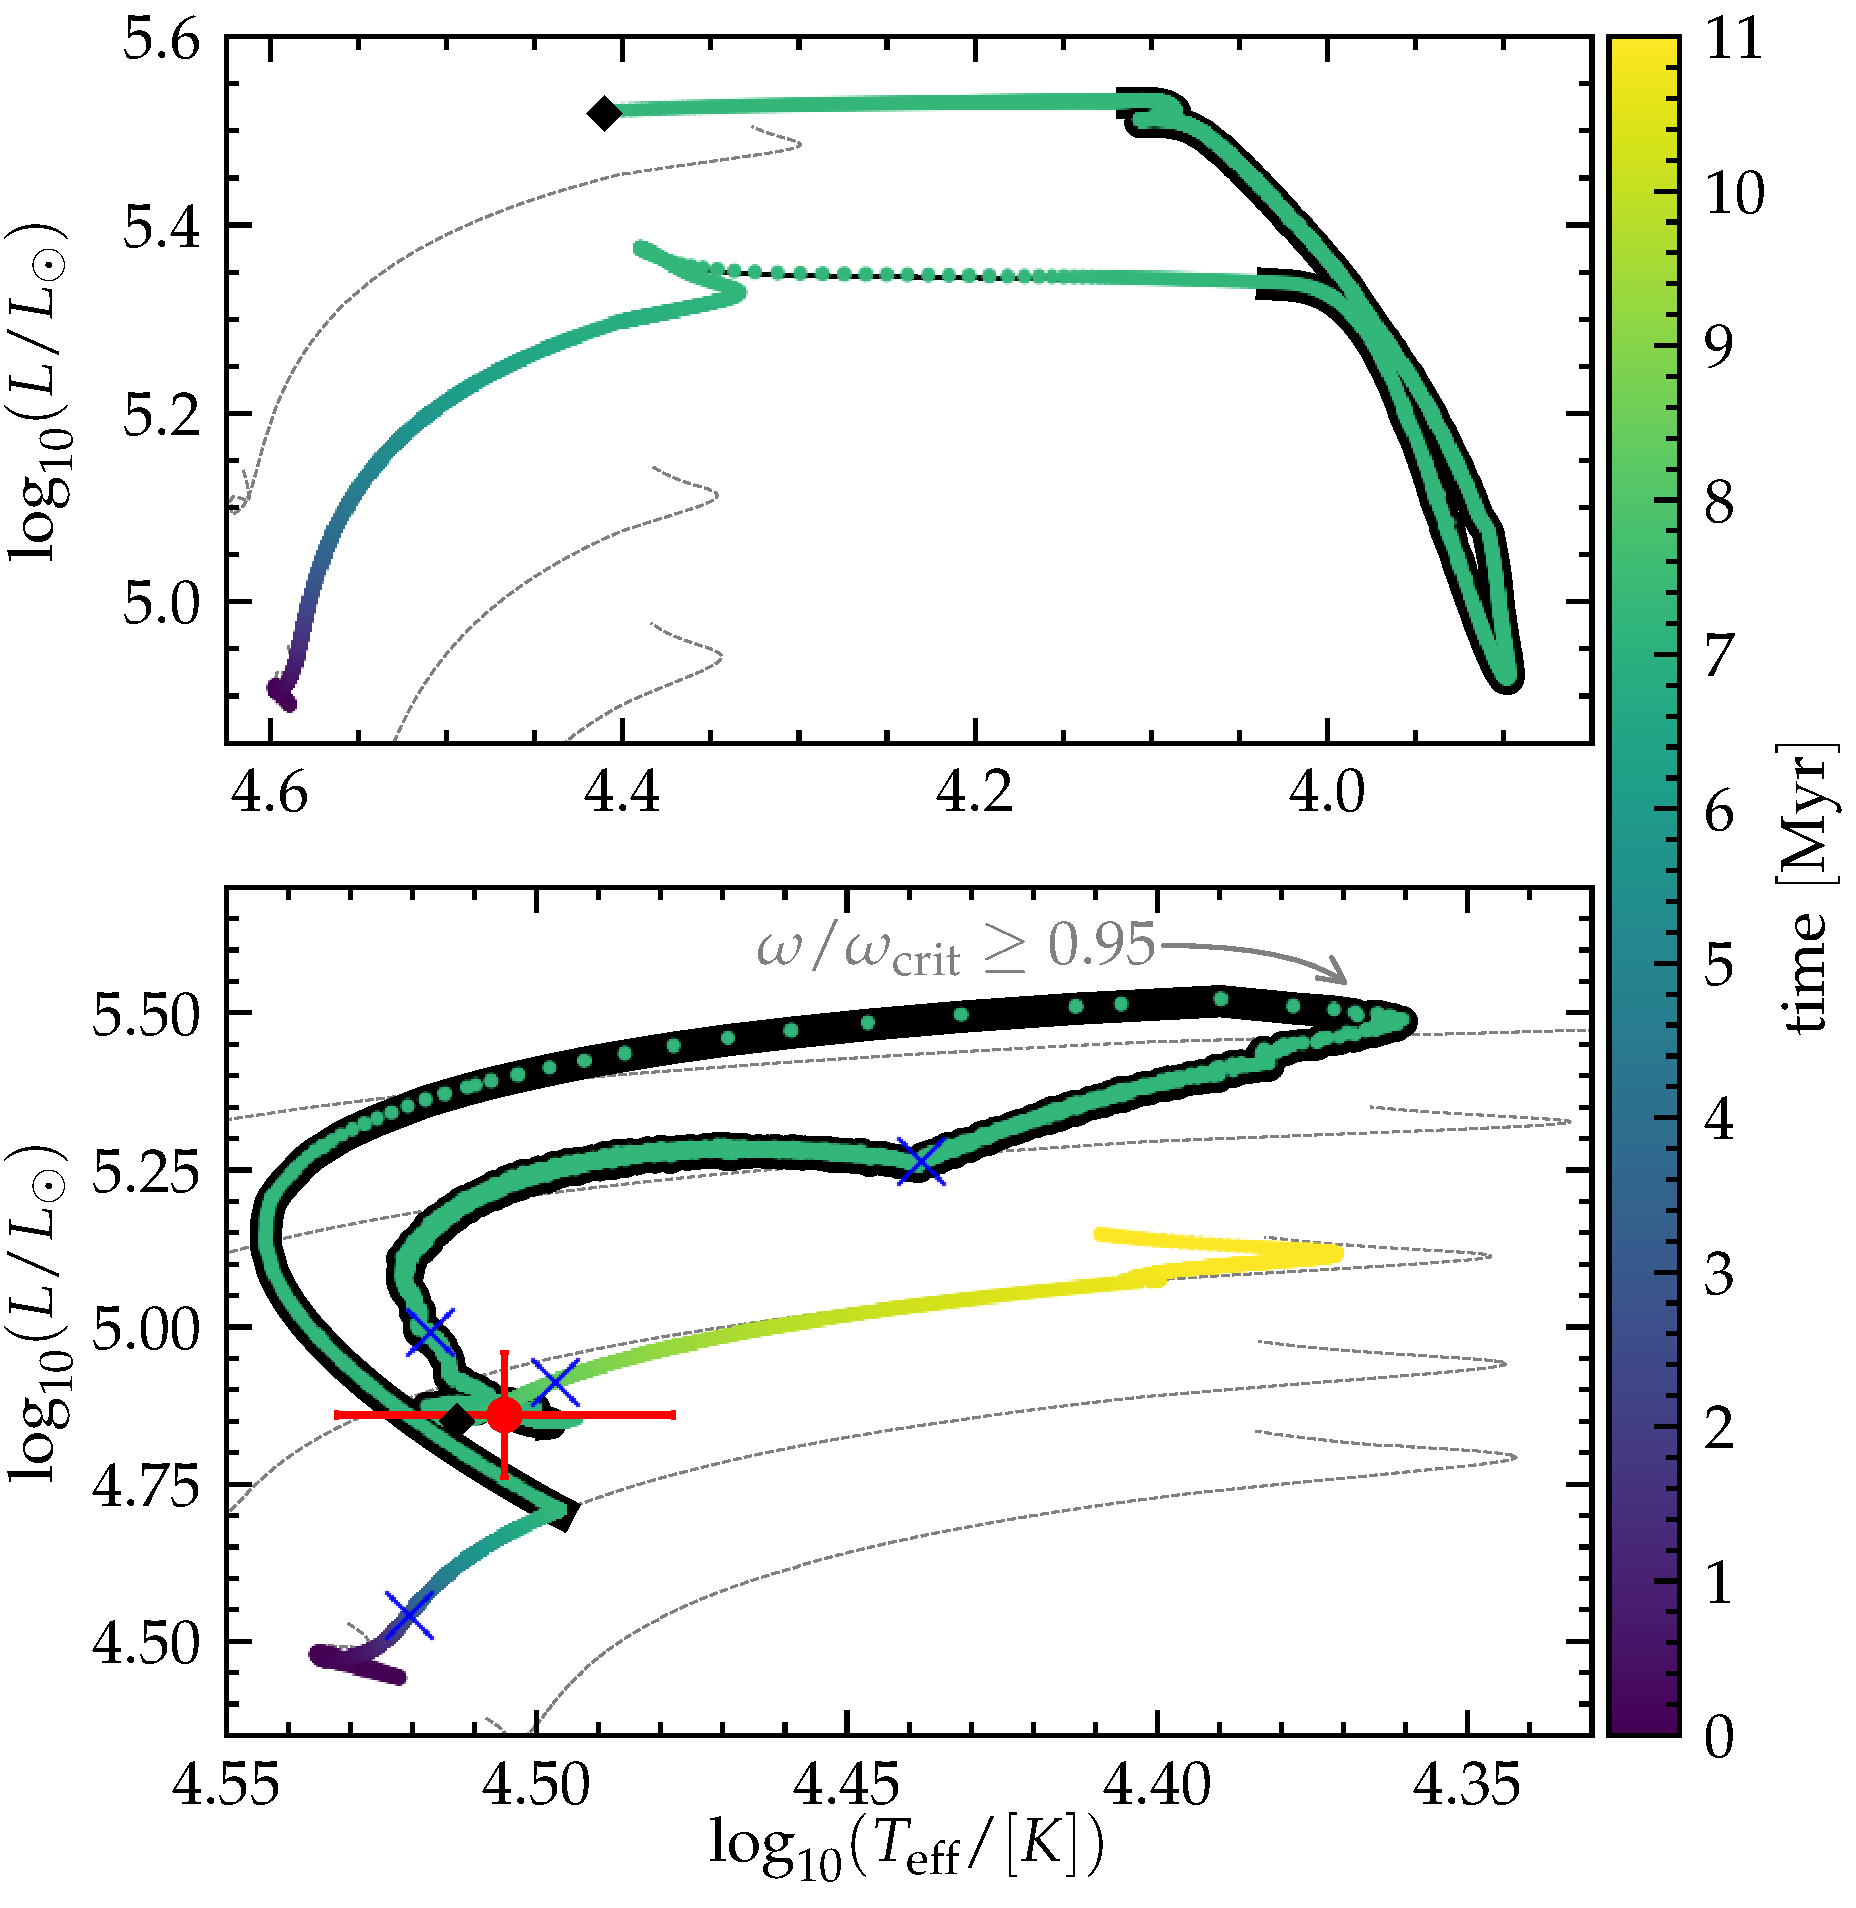
\includegraphics[width=0.5\textwidth]{HRD_both}
  \caption{HRD for the donor star (top) and accretor star (bottom) of
    the progenitor binary of \zoph. Each point is separated by 50
    years of evolution. The colors represent the
    stellar age, the red datapoint shows the position of \zoph\
    according to \citetalias{villamariz:05}, thin blue crosses mark the
    position of the profiles shown in \Figref{fig:D_mix}, and the black diamonds mark the
    position at the end of the binary run. We continue the accretor
    evolution as a single star from there until core H depletion,
    hence the bottom panel shows a longer time. We emphasize the different
    scales on the two panels. The thin gray dashed line show the main
    sequence evolution of non-rotating single stars of 15, 17, 25, and
    30\,$M_\odot$ at $Z=0.01$ for comparison.}
  \label{fig:HRD_both}
\end{figure}


We describe here the evolution of a binary system where the accretor
star can broadly reproduce all the observed features of \zoph. We assume initial masses
$M_1=25\,M_\odot$, $M_2=17\,M_\odot$ on a period of $100$\,days at
$Z=0.01$.

\Figref{fig:HRD_both} shows the Hertzsprung-Russell diagrams (HRD)
of both stars. After $\sim$$7.24$\,Myr, the donor star (top panel) evolves off the main
sequence and $\sim8400$\,years later, when the donor's effective
temperature reaches about $T_\mathrm{eff}\simeq 10^4$\,K, mass transfer starts. This
results in a stable case B RLOF. We refer to \cite{gotberg:17, laplace:21, blagorodnova:21}
and references therein for a detailed description of the evolution of
massive donor stars in binaries. Although our models are
more massive, the qualitative behavior of the donor star is similar.

At the onset of RLOF, the accretor star (bottom panel of
\Figref{fig:HRD_both}) is still on the main sequence with
$T_\mathrm{eff}\simeq10^{4.5}$\,K. Because of accretion,
it quickly becomes over-luminous ($L\simeq10^{5.4}\,L_\odot$), and its
radius increases dramatically from $\sim7.5\,R_\odot$ to
$\sim35\,R_\odot$. Once the accretor reaches critical rotation
(roughly at the lowest $T_\mathrm{eff}$ in the bottom panel of
\Figref{fig:HRD_both}), the star begins contracting and its
$T_\mathrm{eff}$ increases. At $T_\mathrm{eff}\simeq 4.{43}$\,K the
material transferred from the companion star becomes progressively
more He-rich, causing a ``v-shaped'' feature in the evolutionary
track. This indicates that the partially processed outer layers of the donor's core are
uncovered by mass transfer. %  after the convective core recession in
% mass during the main sequence.
This late mass transfer puts material at high mean molecular weight
$\mu$ on top of the primordial envelope of the accretor, modifying the morphology of the evolutionary track. Thermohaline mixing starts in the outer layers of the accreting star, and, together with rotational mixing, it progressively dilutes the surface He and N mass fractions and causes noisy features on the HR diagram \citep[e.g.,][]{cantiello:07}. \Secref{sec:mixing} describes in more detail the mixing processes inside the accretor, we emphasize here that the algorithmic choices made to model mixing (and rotation) might impact the morphology of the accretor's evolutionary track during RLOF. However, the entire duration of RLOF (and thus of the feature in the bottom panel of \Figref{fig:HRD_both} from the departure from the main-sequence to the black diamond) is only about
$10^4$\,years.

We evolve the binary system until the black diamonds in
\Figref{fig:HRD_both}, which occurs well after the donor detaches from
the Roche Lobe. At this point, the accretor is a H-rich fast-rotating
star of
$\sim$$20.1\,M_\odot$. Available mass estimates for the presently single \zoph\ are highly uncertain, but most include
$20\,M_\odot$ (e.g., \citealt{hoogerwerf:01}, \citetalias{villamariz:05}, \citealt{neuhauser:20}). The accretor's post-RLOF orbital velocity is
$v_2\simeq40\,\kms$, which is expected to decrease a bit further due to wind-driven widening of the binary, but is in good agreement with the presently observed runaway velocity of \zoph.

Accounting for both wind mass loss and the amount of mass transferred, at the end of RLOF the donor becomes a He star of
$\sim$$9.4\,M_\odot$, likely to contract further and appear as a
Wolf-Rayet star. It's surface H mass fraction is $\lesssim 0.2$ and
most of the H is likely to be removed by further wind mass loss
\citep[e.g.,][]{gotberg:17}. \todo{Ylva: want to expand?}.
\todo{maybe move next paragraph to discussion?} For our assumed
scenario to work, such donor needs to successfully explode in a SN,
breaking the binary system and making a neutron star remnant. While
the post-RLOF donor mass we obtain is rather high, recent studies
suggest higher ``explodability'' of donor stars in binary systems
\citep[e.g.,][]{schneider:21, laplace:21, vartanyan:21}. Furthermore,
neither the initial donor mass $M_1$ nor the initial period are observable,
and thus there is room to chose different values to obtain easier to
explode donors and faster (or slower) accretors post-RLOF.

From the black diamond onwards, we evolve the accretor as a single star with the same \texttt{MESA} setup until TAMS. The main-sequence track on which the accretor settles post-RLOF has a higher luminosity compared to the original track because of the accretion of mass, and it has also a slightly different slope due to the close-to-critical rotation and the accretion of partially nuclearly processed material (He- and N-rich) material.

The red errorbars in the bottom panel of \Figref{fig:HRD_both} mark the approximate position of \zoph\ based on the analysis of \citetalias{villamariz:05}. The color of the track in \Figref{fig:HRD_both} indicate that our accreting star spends about
$\sim$2\,Myr within the represented errorbars after the end of RLOF. Assuming the kinematic age of
$1.78\pm0.21$ \citep{neuhauser:20}, and estimating a remaining lifetime of the donor of
$\sim$0.5\,Myr, this gives the correct timescale for the binary SN scenario.
The observed position of \zoph\ on the HRD, and especially
its relatively high $T_\mathrm{eff}$ would be hard to reproduce
assuming initially less massive accretors (which would remain too cool
even after accreting mass), or more equal initial mass ratio (which
would produce a too evolved accretor at the onset of mass transfer).

\begin{figure}[htbp]
  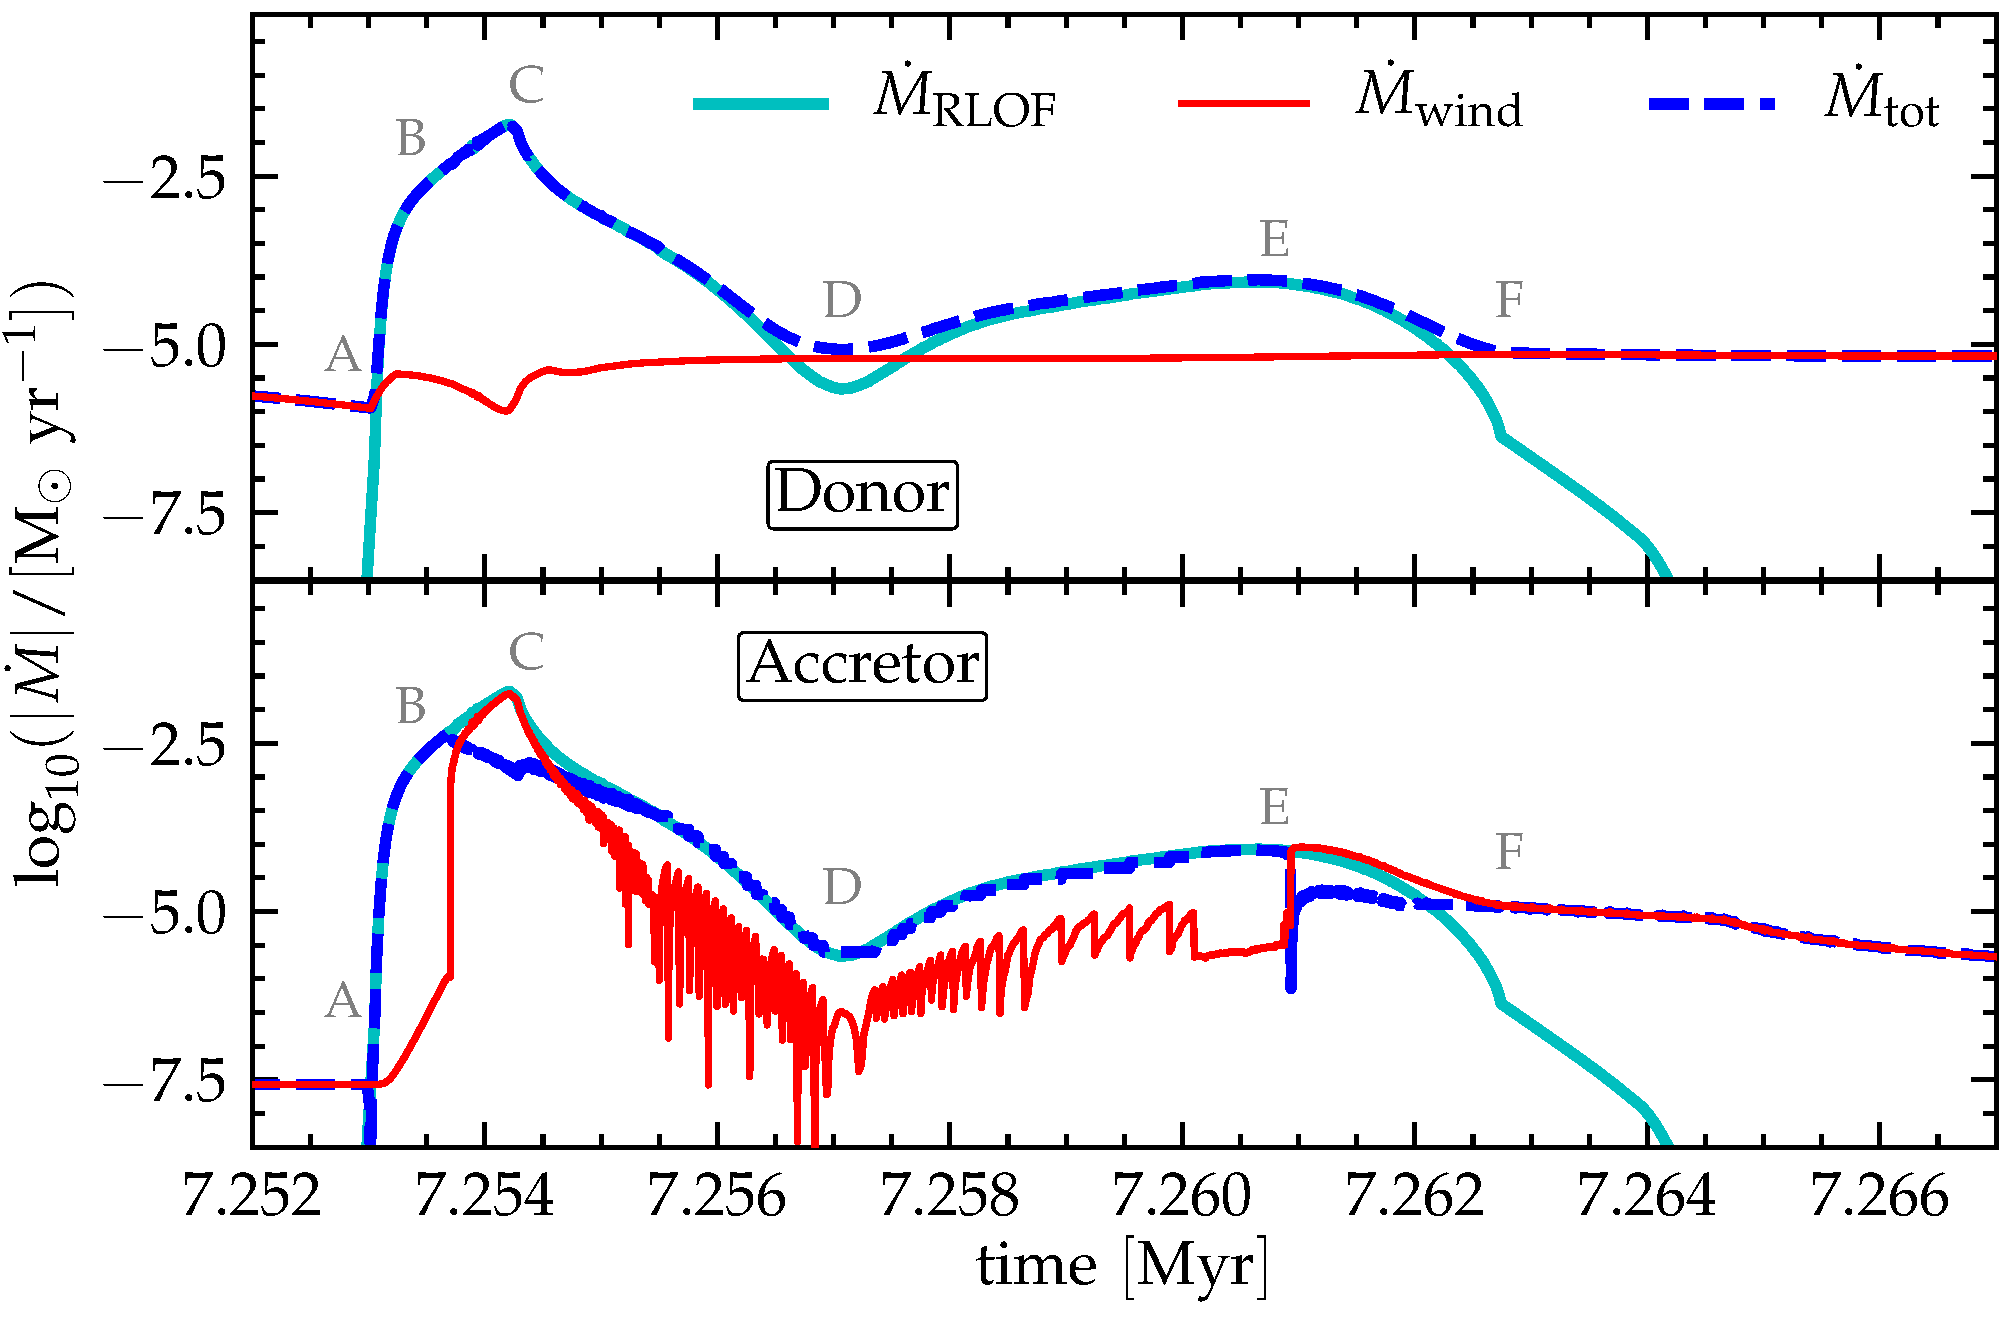
\includegraphics[width=0.5\textwidth]{MT}
  \caption{Mass transfer rates as a function of time during RLOF. The top (bottom) panel
    shows the donor (accretor) star. The cyan solid lines show the
    mass transfer rate between the two stars. The dashed blue lines
    show the actual change in the mass of the stars (due to the
    combination of wind, and accretion efficiency). The thin red
    lines show the wind mass loss rates. During RLOF the accretor
    reaches critical rotation, which leads to oscillations in the
    rotationally-enhahnced wind mass loss.}
  \label{fig:MT}
\end{figure}

\Figref{fig:MT} shows the rate of mass change for each star
during RLOF. The top panel focuses on the donor star
which loses mass to RLOF (cyan line) and wind mass loss (thin red
line). The dashed blue lines show their combination resulting in the
actual rate of mass change of the stars.
The bottom panel shows instead the accreting star, which grows in mass
because of the mass transfer. At peak the mass transfer rates reaches very high
values above $10^{-2.5}\,M_\odot\ \mathrm{yr^{-1}}$, and taps into the
optically thick matter of the donor.

During RLOF, the total amount of mass lost by the donor is
$\Delta M_\mathrm{donor} \simeq 10.6\,M_\odot$, of which only
$\Delta M_\mathrm{accretor}\simeq 3.4\,M_\odot$ are successfully
accreted. This corresponds to an overall mass
transfer efficiency
$\beta_\mathrm{RLOF}\equiv \Delta M_\mathrm{accretor}/\Delta M_\mathrm{donor} \simeq 0.3$,
although the accretion efficiency is \emph{not} constant throughout the
mass transfer \citep[e.g.,][]{vanrensbergen:06}, instead it depends on the radial and rotational evolution of
the accreting star.

At the end of RLOF, the donor star briefly expands again
($T_\mathrm{eff}\simeq10^{4.1}$\,K, $L\simeq10^{5.5}\,L_\odot$). This
is due to the partial recombination of the now He-rich outer layers,
which causes a transient surface convection layer. This causes the
second broad peak in the mass transfer rates centered at $7.261$\,Myrs. We
find this to be the culprit of difficulties in modeling massive
binaries transferring mass in older \texttt{MESA} releases, because
although only a very small amount of mass is involved, this would lead
to large radial expansion much beyond the donor's Roche lobe, and
cause numerical problems.

The wind mass loss (in red) controls the accretion efficiency and thus
the difference between the actual rate of change in mass of the
accretor (thick dashed blue) and the rate at which mass is being
transferred. At peak, where the red and the cyan lines overlap, mass
transfer becomes very non-conservative, but for most of the evolution
the (rotationally enhanced) wind removes only a fraction of the
accreted mass. The interplay between the stellar radius and rotation
causes the oscillations visible in the bottom panel, whose amplitude
is generally lower than the RLOF mass transfer rate.

\subsection{Internal mixing and surface composition of the accretor}
\label{sec:mixing}

\begin{figure*}[htbp]
  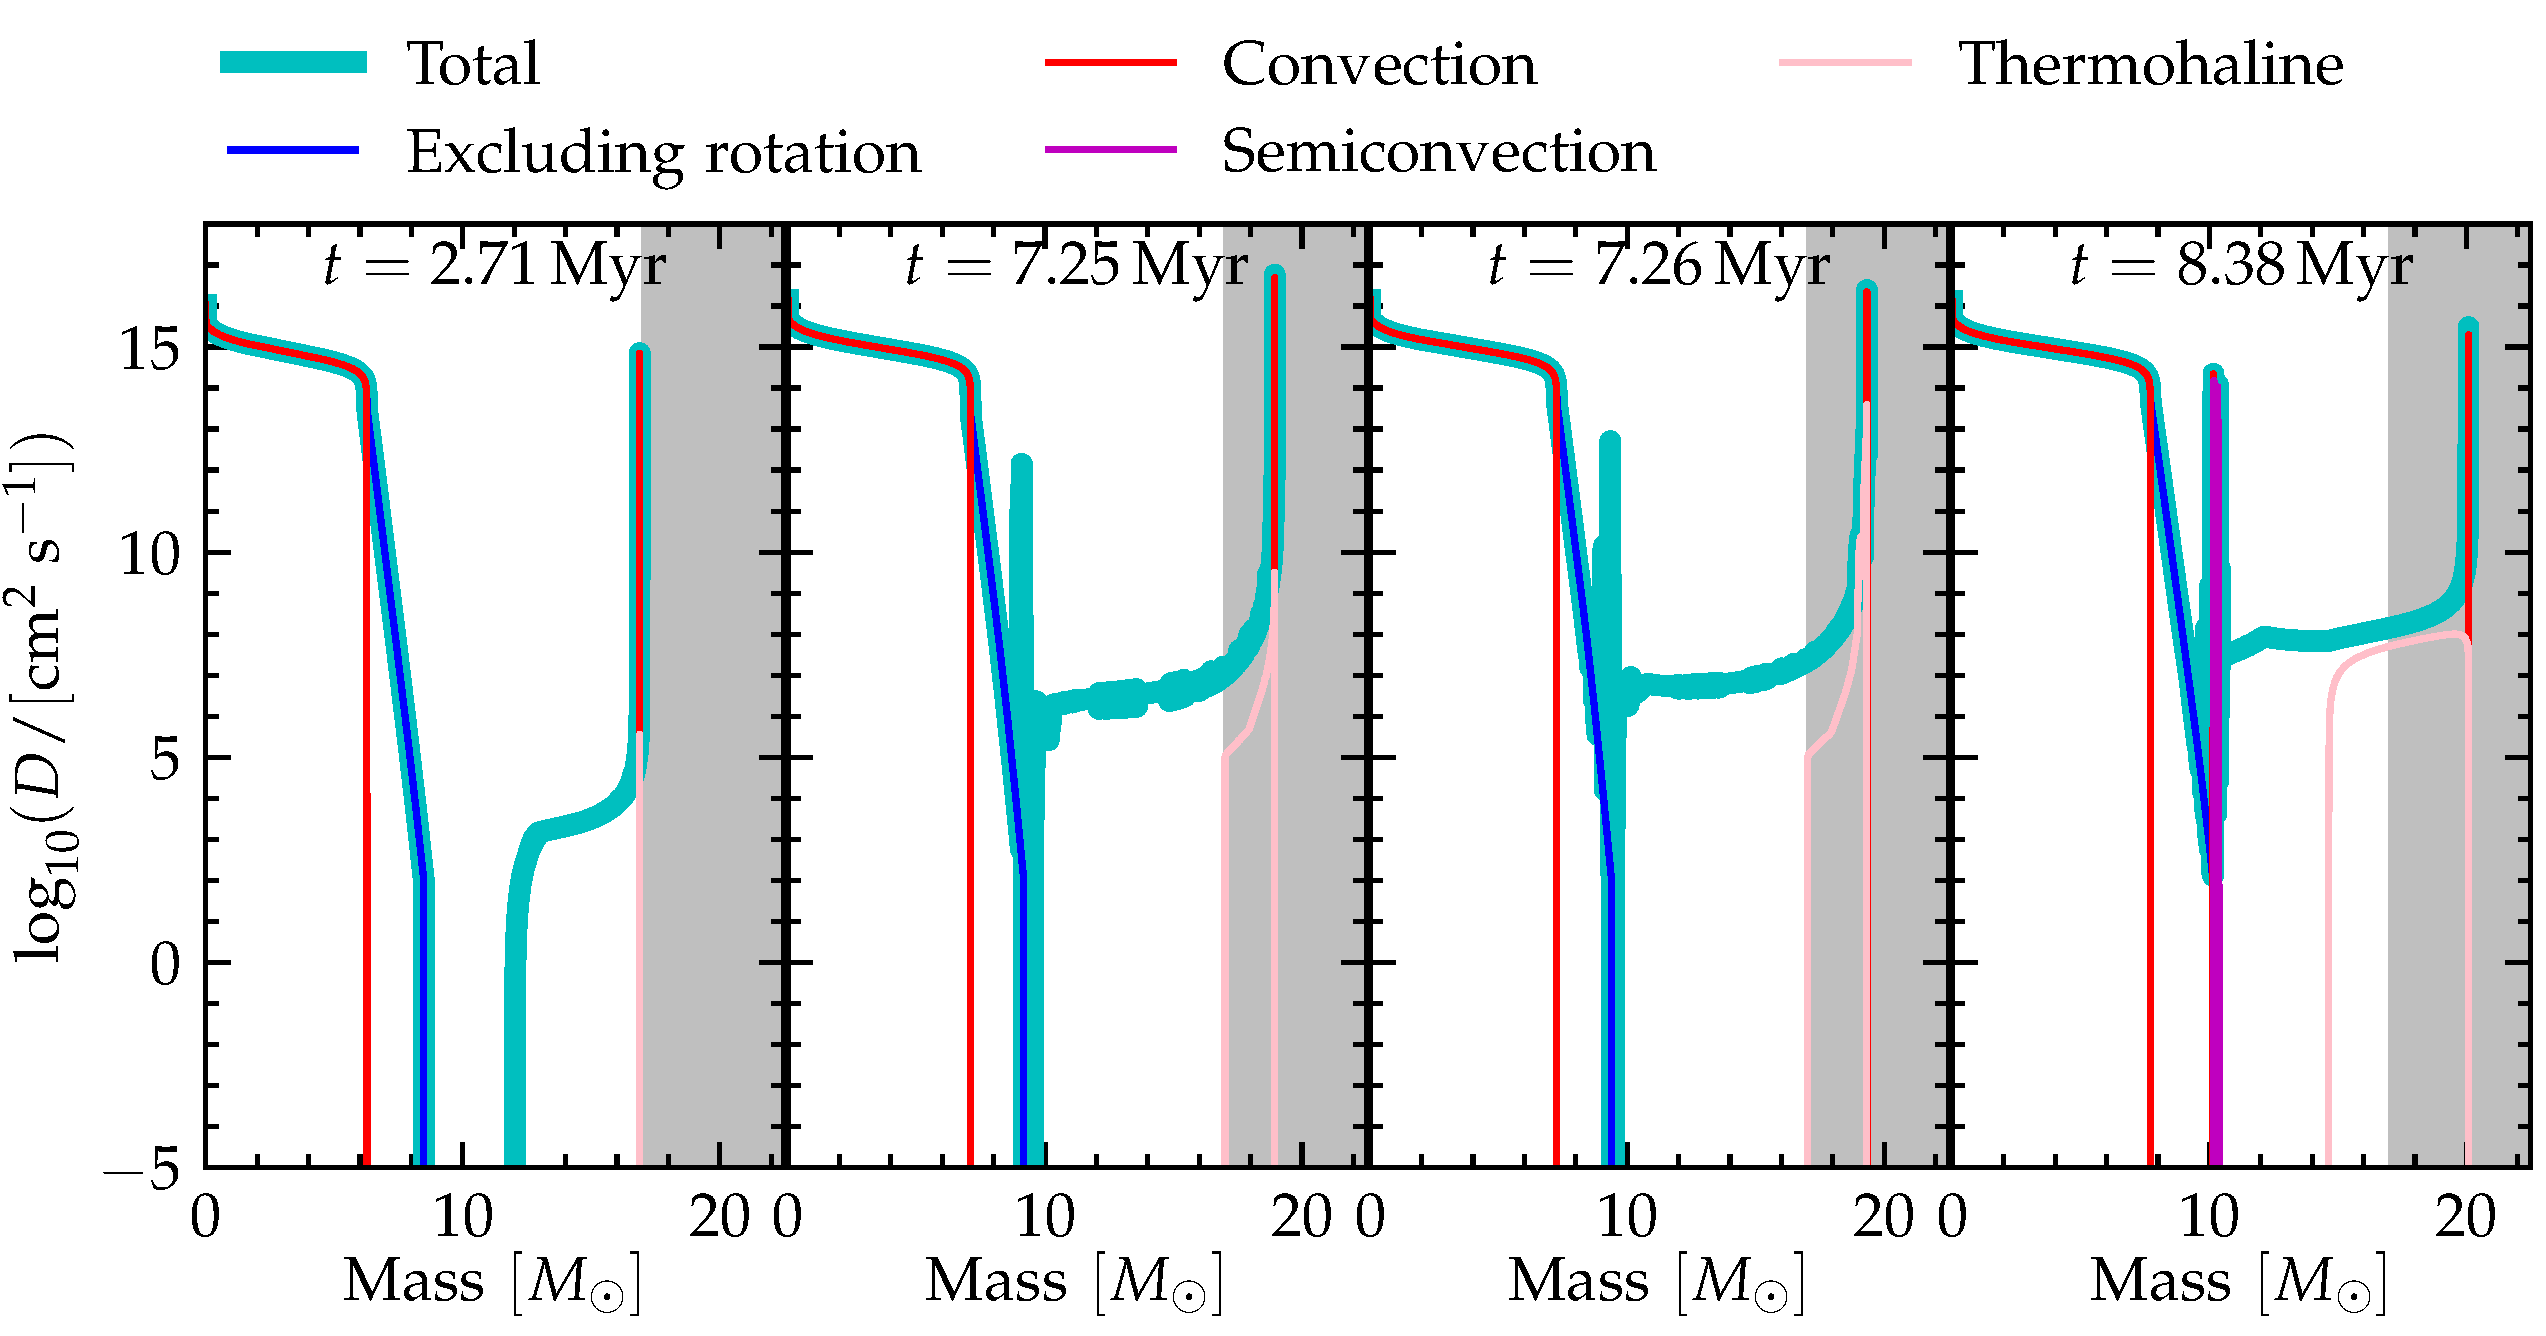
\includegraphics[width=\textwidth]{D_mix}
  \caption{Mixing diffusion coefficients in the accretor star. From
    left to right, each panel shows times during the main sequence
    ($t$=2.71\,Myr), right before the ``v-shaped'' feature during RLOF
    ($t$=7.25\,Myr), close to the end of RLOF ($t$=7.26\,Myr), and
    after mass transfer ($t=8.38$\,Myr). The total diffusion
    coefficient (thick cyan line) is obtained as the sum of
    non-rotational mixing processes (i.e., here overshooting, thin
    blue line), convection (shown in red), thermohaline mixing (pink)
    and semiconvection (in purple). The gray area corresponds to mass
    accreted during RLOF. The HRD position for each panel is marked by
    a thin blue cross in \Figref{fig:HRD_both}.}
  \label{fig:D_mix}
\end{figure*}

\texttt{MESA} treats mixing processes in the diffusion approximation \citep{paxton:11}.
To illustrate the dominant processes throughout the
accretor's evolution, we show in \Figref{fig:D_mix} the diffusion
coefficients as a function of mass coordinate at selected times. Each
panel corresponds to one of the thin blue crosses in the bottom panel
of \Figref{fig:HRD_both}, and the gray shaded areas mark mass that is
accreted during RLOF. The last panel roughly represents the predicted
internal structure of \zoph\ as observed today.

In \Figref{fig:D_mix}, the thin red lines correspond to convection,
with the initial convective core of
$\sim$$6\,M_\odot$ clearly visible in the first panel. In all models, a tiny sub-surface convective region is also visible in the outermost layers (see e.g., \citealt{cantiello:21}).  The thin blue lines mark mixing processes that are not related to rotation, nor are any of the other processes explicitly shown, which here effectively means overshooting. The extension of the diffusion coefficient above the convective core in all panels is the typical behavior for an exponentially decreasing overshooting. Purple and pink represent semiconvection and thermohaline mixing, respectively. Before mass transfer (left-most panel), only a small amount of sub-surface thermohaline mixing occurs, with a mass extent comparable or smaller to the sub-surface convective zone, and no semiconvection occurs. The thick cyan line corresponds to the total diffusion coefficient, obtained as the sum of the diffusion coefficients for each process modeled: where the cyan line is not overlapping with the others, rotational mixing (and more specifically Eddington-Sweet meridional circulation) is the dominant process.

During RLOF (second and third panel), the spin up due to accretion causes an increase in the rotational mixing (cyan line in the outer layers), and the accretion of nuclearly processed material progressively widens the thermohaline mixing region at the surface. Late during the mass transfer (third panel), thermohaline mixing dominates the outermost layers -- except within the sub-surface convective zone, but throughout most of the envelope rotation does the lion's share of the mixing. Thermohaline mixing and Eddington-Sweet circulations together mix inwards and dilute the CNO-enriched material coming from the donor's surface.

At the same time, the increase in the accretor mass drives
rejuvenation \citep[e.g.,][]{schneider:16}. This can be seen as a
growth of the convective core from
$\sim$$6\,M_\odot$ to almost $\sim$$8\,M_\odot$, plus the
corresponding growth of the overshooting region. This mixes inward
H-rich material resulting in an elongation of the accretor's lifetime,
and at the same time mixes outward CNO-equilibrium matter, connecting
the N-rich core with the outer envelope polluted from the top.


    % this table was automatically generated using the table.ipynb in the repository associated to this manuscript
    \begin{table*}[hbpt]
    \centering
    \begin{tabular}{c|c|c|c|c|c|c|c|c}
    \hline\hline
    $M \ [M_\odot]$ & $R\ [R_\odot]$ & $\log_{10}(\omega / [\mathrm{s^{-1}}])$ & $v_\mathrm{rot} \ [\kms] $ & $X(^{1}\mathrm{H})$ & $X(^{4}\mathrm{He})$ & $X(^{12}\mathrm{C})$ & $X(^{14}\mathrm{N})$ & $X(^{16}\mathrm{O})$ \\
    \hline
    20.1 & 9.6 & -4.263 & 366.1 & 0.678010 & 0.312093 & 0.001344 & 0.001340 & 0.004148 \\
    \hline
    \end{tabular}
    \caption{Properties of the accretors shortly after the end of RLOF
    (last thin blue cross in \Figref{fig:HRD_both})}
    \label{tab:surf_prop}
    \end{table*}
    


\Tabref{tab:surf_prop} summarizes the surface properties of the
accretor star at the time shown in the last panel of
\Figref{fig:D_mix}, that is shortly after the RLOF phase, while the
model is still roughly at the observed position of \zoph.

Both the mass and radius agree reasonably well with the estimates from
\citetalias{villamariz:05} and previous studies, i.e.~$20\,M_\odot$ and
$8.3\pm1.5\,R_\odot$, respectively. The surface rotational velocity in
excess of $350\,\kms$ is also in the correct ballpark albeit possibly
on the low end. We discuss further rotation and angular momentum
transport in \Secref{sec:rot}. We report the surface H mass
fraction\footnote{This is needed to convert mass fractions reported
  here into $\varepsilon(X)=12+\log_{10}(N_X/N_H)$, where $N_X$ and
  $N_H$ are the number fractions of species $X$ and H, respectively.},
lower than primordial because of the accretion of nuclearly processed
material, and the surface mass fraction of the most prominent species
$^4\mathrm{He}$, $^{12}\mathrm{C}$, $^{14}\mathrm{N}$,
$^{16}\mathrm{O}$.  Assuming our surface H mass fraction
$X(^1\mathrm{H})$, the corresponding mass fractions of $^4\mathrm{He}$,
$^{12}\mathrm{C}$, $^{14}\mathrm{N}$, $^{16}\mathrm{O}$ reported in
\citetalias{villamariz:05} are
$0.33^{+0.14}_{-0.05}$,
$0.0006\pm0.0004$,
$0.002\pm0.001$, and
$0.005\pm0.004$.  Our values are
sensitive to the interplay between several poorly understood
processes treated in one dimension: mass accretion efficiency, rotationally enhanced wind mass
loss, thermohaline, and inward rotational mixing. Therefore, although
not perfect, we consider the match with the mass fractions reported by
\citetalias{villamariz:05} surprisingly satisfactory.

We now compare the mixing processes
happening in a single rotating massive stars and in our accretor
model. \Figref{fig:n14} shows the mass fraction of $^{14}\mathrm{N}$
as a function of mass coordinate along the evolution of three
$20\,M_\odot$ stars initialized with
$\omega/\omega_\mathrm{crit}=0.2,0.3,0.4,0.5$ where $\omega$ is the
surface angular frequency and
$\omega_\mathrm{crit}=\sqrt{(1-L/L_\mathrm{Edd})GM/R^3}$ and
$L_\mathrm{Edd}$ is the Eddington luminosity computed using the
stellar opacity from the outermost mesh point down to optical depth
$\tau=2/3$, $L$ is the luminosity, $G$. These rotating single stars have an otherwise identical
setup as our binary model. The last panel of \Figref{fig:n14} shows
our accretor model. The dotted red line marks the primordial mass
fraction of $^{14}\mathrm{N}$ for the adopted $Z=0.01$, the thin
dashed lines mark the surface value at TAMS. The colored tracks show
selected profiles throughout the main sequence, with lighter colors
corresponding to more evolved stars.


The solid red line and red shaded area across all panels show the
$^{14}\mathrm{N}$ from \citetalias{villamariz:05} (assuming the
surface mass fraction from our model listed in \Tabref{tab:surf_prop}): the mass fraction of $^{14}\mathrm{N}$
alone is not sufficient to distinguish with these models, and already
a moderate $\omega/\omega_\mathrm{crit}\geq0.3$ is sufficient for
models to reach the lower-limit of the error bar.

The typical evolution


\begin{figure*}[htbp]
  \centering
  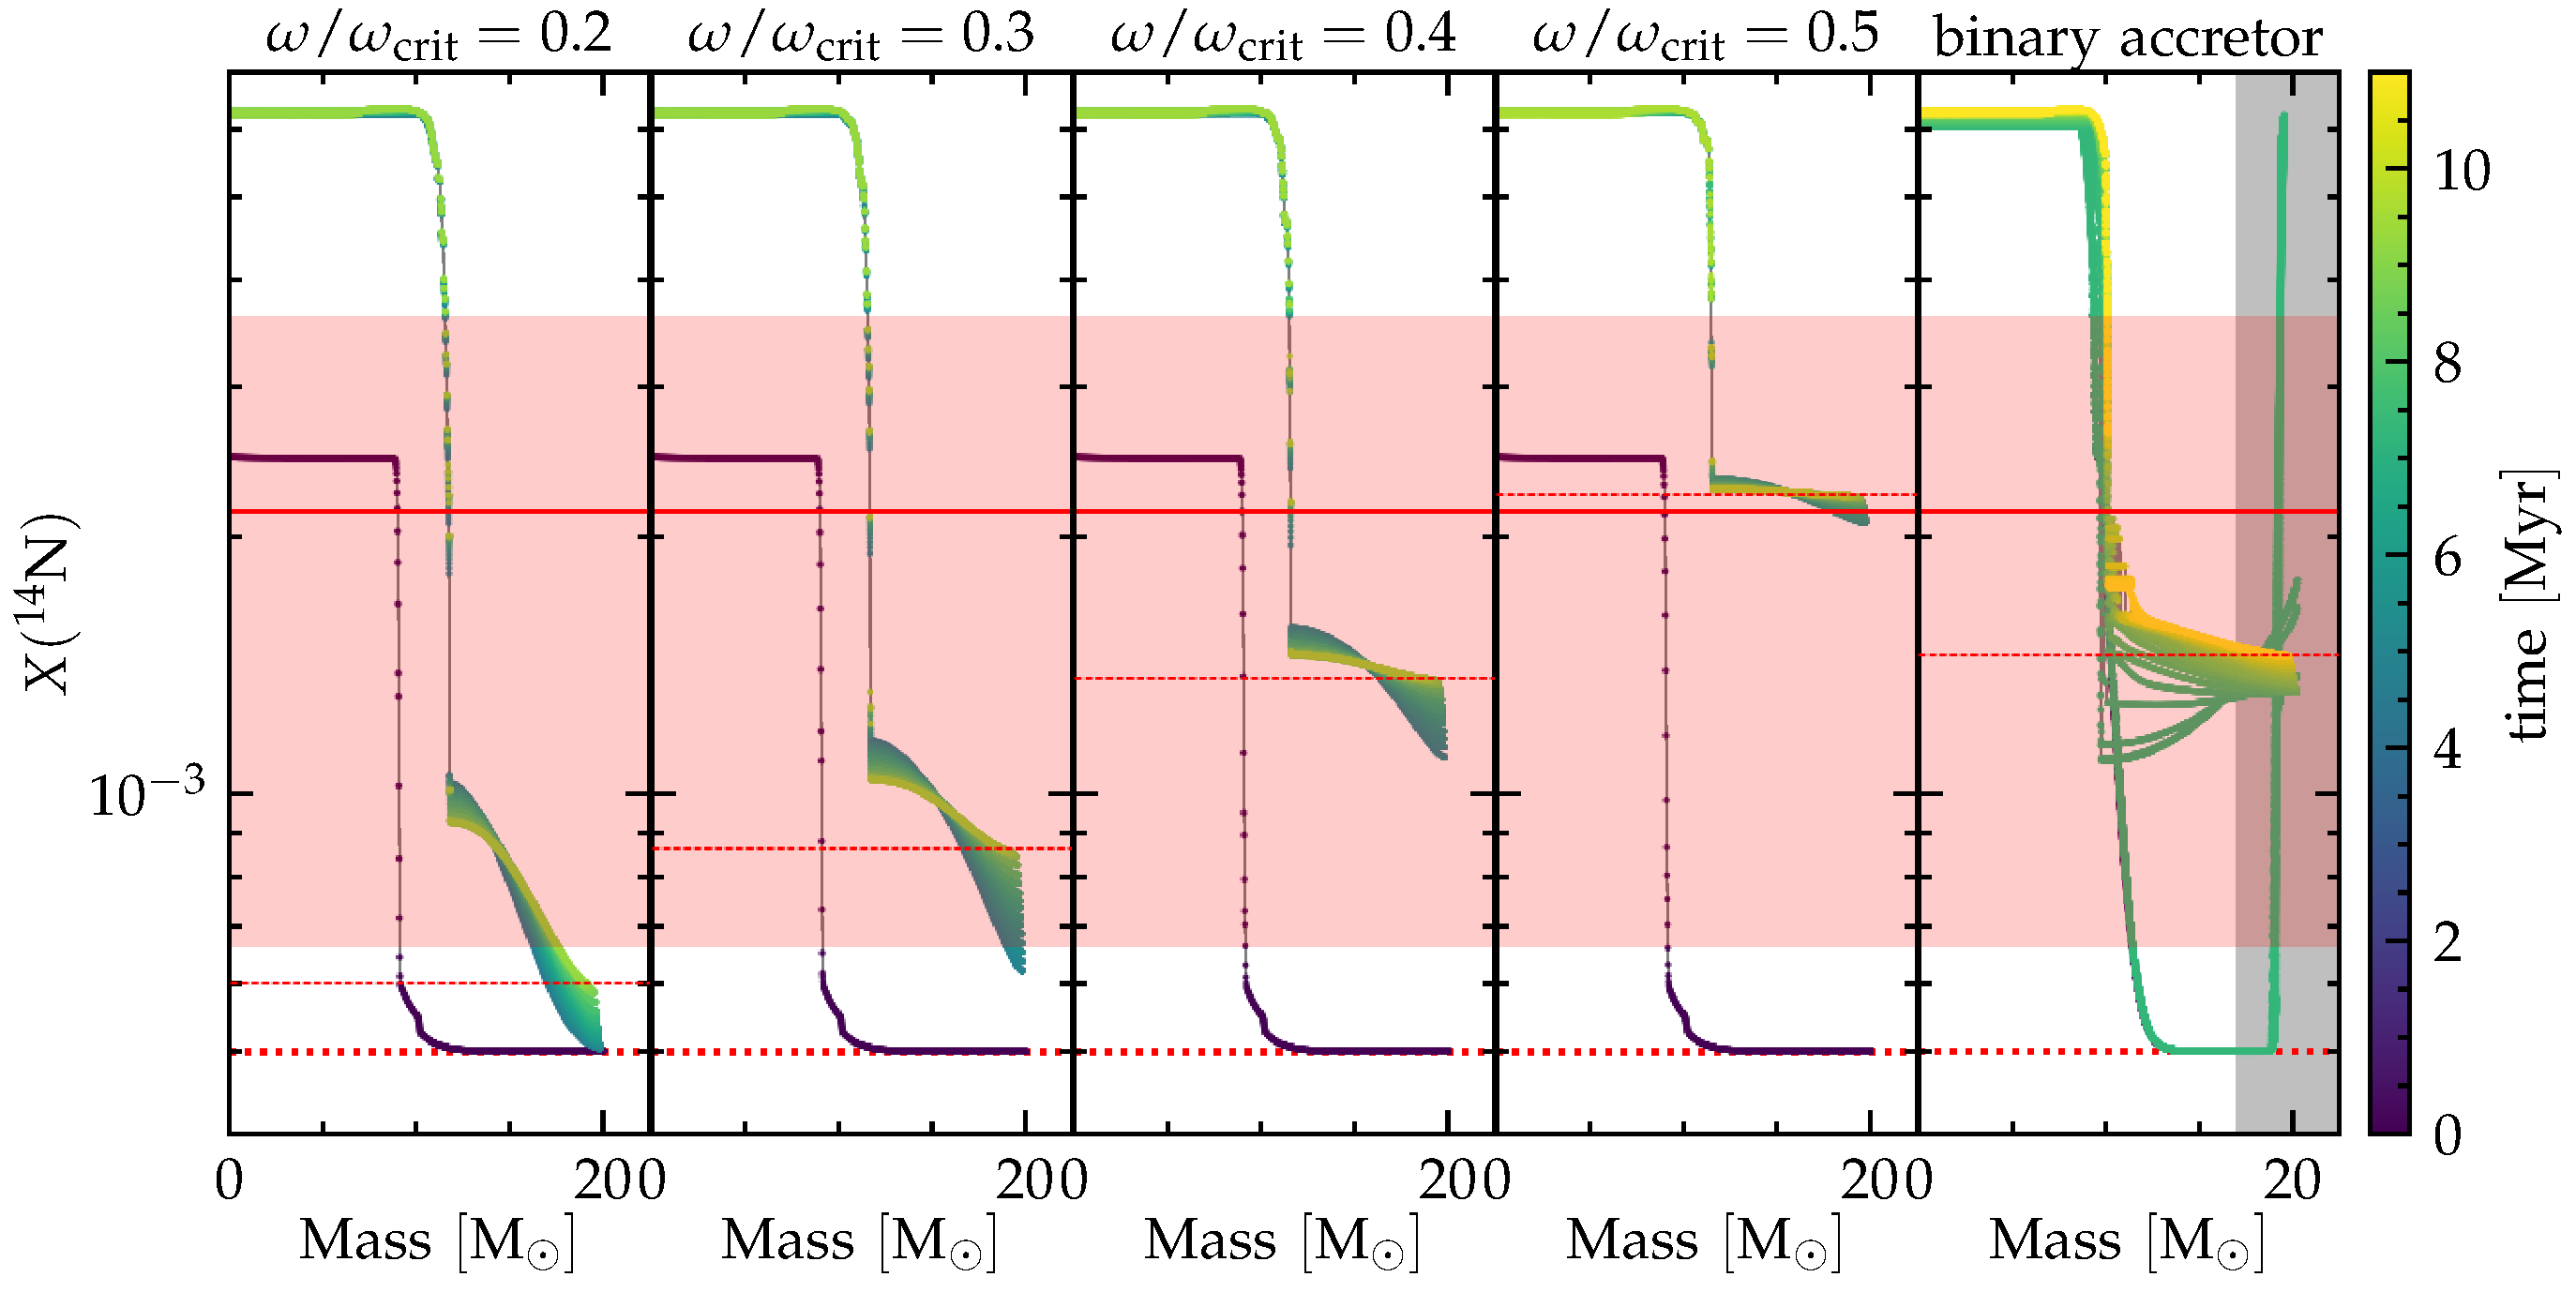
\includegraphics[width=\textwidth]{n14_struct_complete_zeta_ab}
  \caption{$^{14}\mathrm{N}$ mass fraction as a function of mass
    coordinate for $20\,M_\odot$ single star models with increasing
    $\omega/\omega_\mathrm{crit}$ at birth (first four panels), and
    for the accretor of our fiducial binary. The dotted thick red line
    marks the primordial value, the thin dashed red line marks the
    surface value at TAMS. In the last panel, the thin vertical dashed line shows the initial total mass of the accretor. The colors of each profile go from dark to
    light at TAMS, and selected profiles along the main sequence are
    shown. The solid red line and the shaded region correspond to the
    mass fraction of $^{14}\mathrm{N}$ estimated by
    \citetalias{villamariz:05} assuming a surface H mass fraction of 0.7:
    the abundance of $^{14}\mathrm{N}$ alone is not strongly constraining.}
  \label{fig:n14}
\end{figure*}



\subsection{Angular momentum transport and internal structure}
\label{sec:rot}

\todo{discuss rotation rate and radius}

\begin{figure}[htbp]
  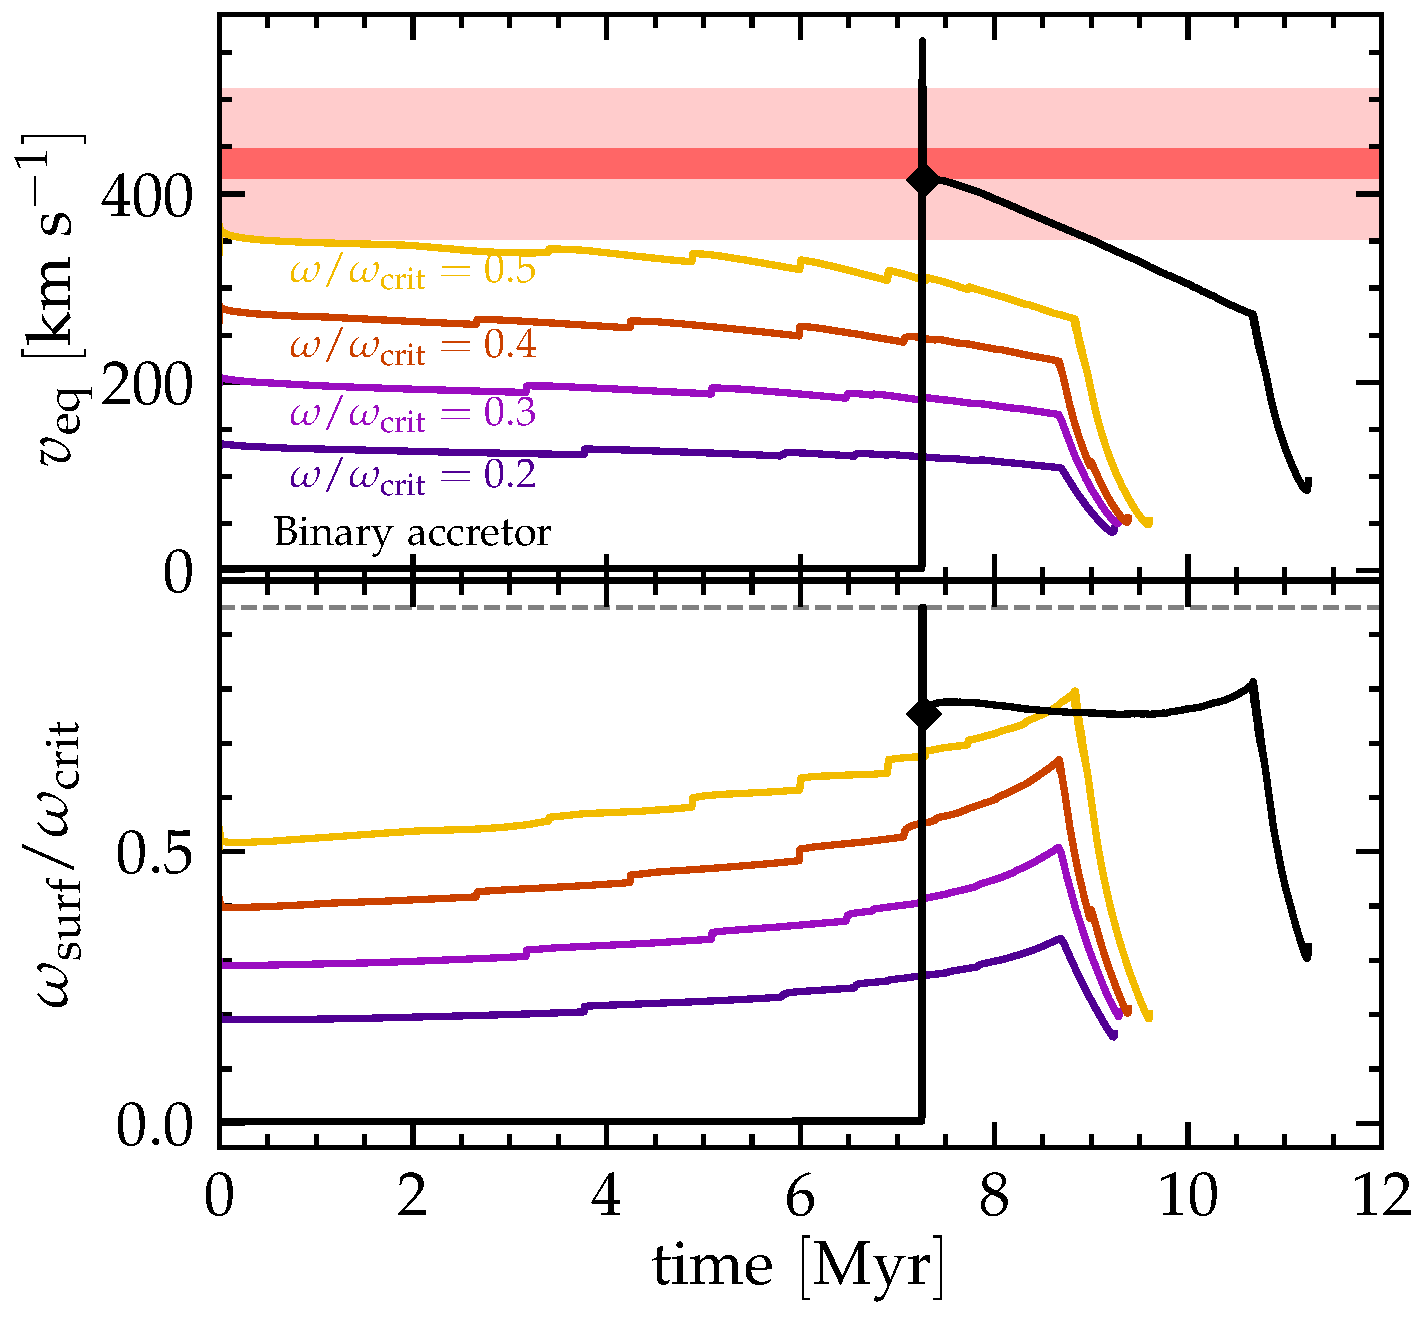
\includegraphics[width=0.5\textwidth]{zeta_rot}
  \caption{Surface averaged rotation rate for the accretor
    model. Shortly after $\sim$7\,Myr the mass transfer quickly spins
    up the accretor at critical rotation. By the time the donor
    detaches from the RLOF the accretor is still spinning at
    $\sim$$400\,\kms$. At this point (beginning of the dot-dashed line), we continue the evolution as a single star, and the accretor quickly spins down. Note however that we use a wind mass-loss rate from \cite{vink:01}, which is observed to be
    $\sim$2 orders of magnitude too high.}
  \label{fig:rot}
\end{figure}


\begin{figure*}[htbp]
  \centering
  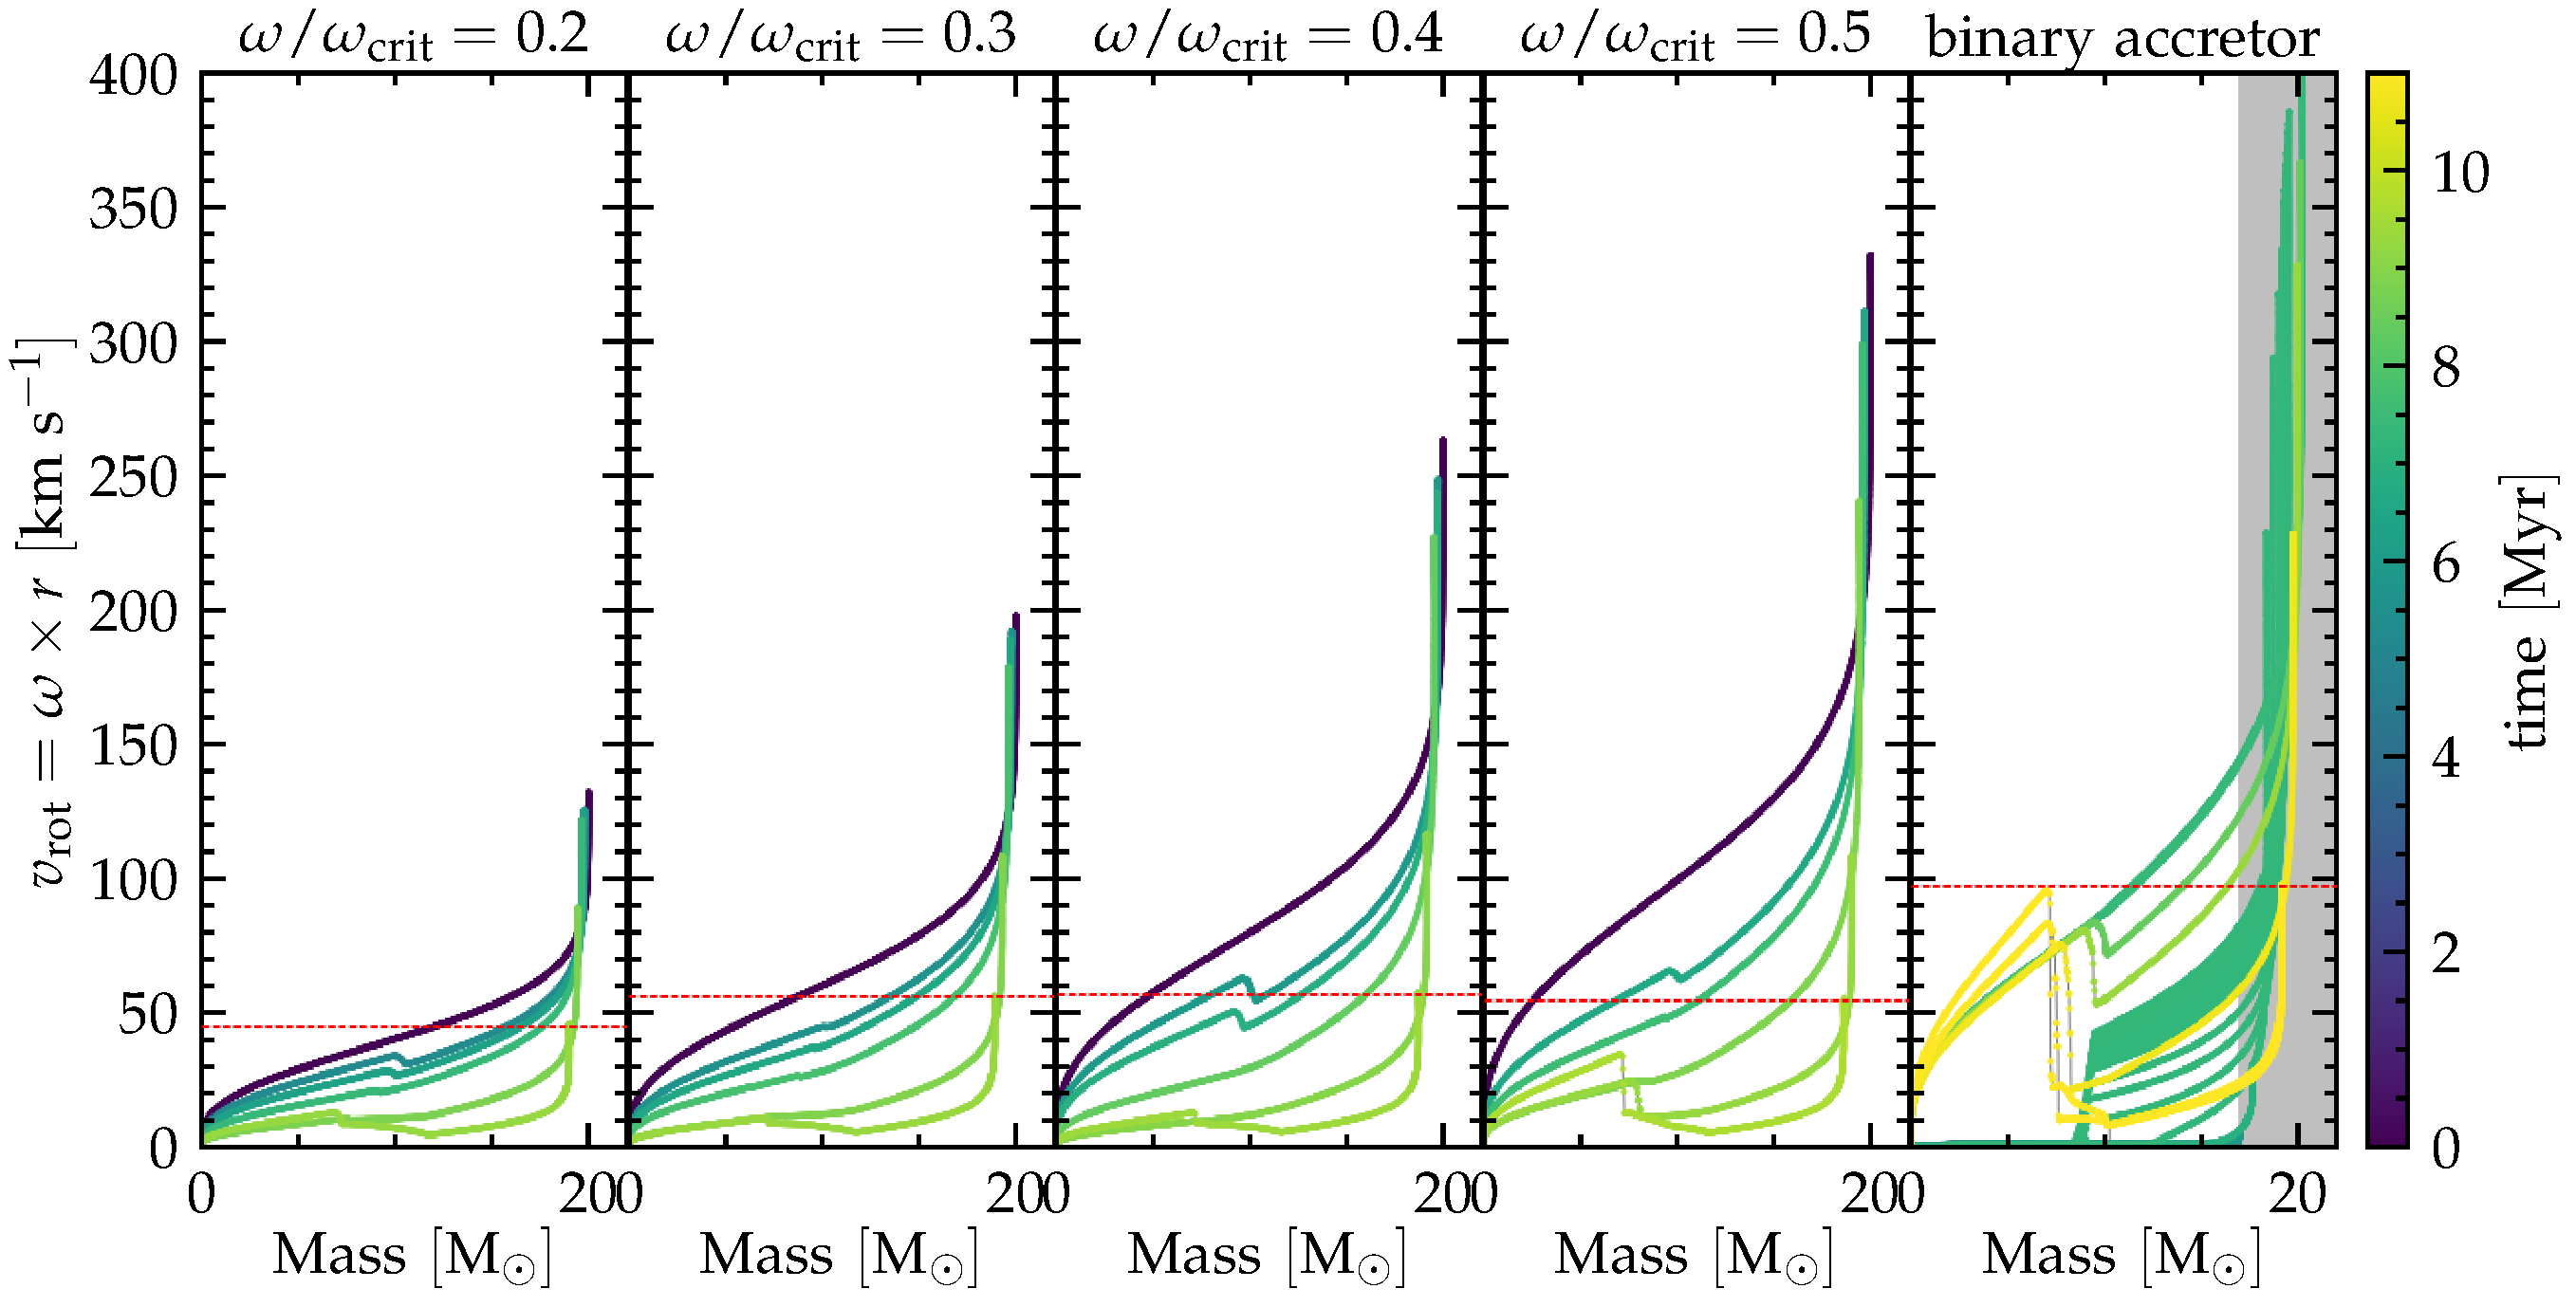
\includegraphics[width=\textwidth]{zeta_Rotational_struct}
  \caption{Internal rotational profile for $20\,M_\odot$ single star models with
    increasing $\omega/\omega_\mathrm{crit}$ at birth (first four
    panels), and for the accretor of our fiducial binary. As in \Figref{fig:n14}, the colors go from dark (close to ZAMS) to light at TAMS, and the thin dashed red line mark the TAMS surface rotation rate. In the last panel, the gray area indicates mass accreted during RLOG. The yellow lines (TAMS) in the last panel show that the core of the accretor is rotating almost as fast as its surface, and both are faster than the surface of single star models.}
\end{figure*}


\section{Robustness of the model}
\label{sec:param_variations}

In this section we investigate the sensitivity of our results to
physical parameters.

\todo{How to present results? Table? Showing what? surface mass
  fractions, rotation, L, Teff}

\todo{
  Binary parameters:
  \begin{itemize}
  \item $M_1$
  \item $M_2$
  \item $P$
  \item J-accretion
  \end{itemize}
}

\todo{
  Single star parameters:
  \begin{itemize}
  \item thermohaline mixing
  \item Eddington-Sweet circulations
  \item metallicity
  \end{itemize}
}

\todo{others?}

\section{Discussion}
\label{sec:discussio}

\subsection{Free parameters in the treatment of mass transfer}
\label{sec:free_param}

We regulate the accretion efficiency through the rotational
enhancement of mass loss \citep[e.g.][]{langer:98}. \todo{maybe move
  $\beta_\mathrm{RLOF}$ here}. However,
\citep{popov:91, paczinski:91} argued that accretion of mass (but no
angular momentum) might be possible even at critical rotation.

\subsection{The explosion of the former companion}
\label{sec:SN_comp}

Throughout this study, we have assumed the ``binary SN scenario'':
after the mass transfer phase, the explosion of the donor breaks the
binary and ejects the accretor with roughly its pre-explosion velocity
\citep[e.g.,][]{renzo:19walk}. This is the fate of the majority of
massive binary systems, and \zoph\ might be the best example of this
scenario \citep[e.g.,][]{blaauw:52, blaauw:61,
  hoogerwerf:00}. \cite{neuhauser:20} suggested not only the companion
successfully exploded producing the pulsar PSR B1706-16, but that the
explosion produced radioactive $^{60}\mathrm{Fe}$ which polluted
Earth. From kinematic and orbital considerations they estimated a
natal kick of $\sim$250\,$\kms$, which would be sufficiently large to
unbind the binary.\todo{check, be more precise}

However, we have so far neglected the impact of the explosion on the
structure of the accretor star. The blast wave will hit the companion
at a \todo{estimate solid angle} causing mass loss -- directly via
ablation and by injecting energy in the envelope, inflating it and
enhancing its wind \citep{wheeler:75, tauris:98, podsiadlowski:03, hirai:18}.

Using 2D hydrodynamic simulations of the star-SN ejecta interactions
in close binaries ($a\lesssim 60\,R_\odot$,
cf. $a\gtrsim 343\,R_\odot$ in our fiducial binary model),
\cite{hirai:18} found that the companion star recovers its pre-explosion
luminosity and effective temperature within a few years to decades,
and the amount of mass removed by the SN shock is $\lesssim10^{-2}\,M_\odot$



\todo{estimate mass loss}


Because of the SN shock, the just ejected new runaway star might
appear bloated and redder (long before it overtakes the slowing SN
remnant). Hydrodynamical simulations of a non-rotating star
with a SN shock suggest that within \todo{X} the star returns
in equilibrium \cite{hirai:18}. The impact of this brief out of
thermal equilibrium phase on the stellar spin should be investigated
further.

The SN ejecta might also pollute the surface of the runaway depositing
processed nuclear material \citep[e.g.][]{przybilla:08}. However,
enhahnced mass loss, and rapid rotating might rapidly dilute the
yields.

\todo{improve this sec.}


On top of the surface abundances, its extreme rotation rate, and the
peculiar space velocity, \zoph\ poses a number of other
puzzles: its wind mass-loss rate is about two orders of magnitude
lower than theoretical predictions (weak wind problem,
\citealt{marcolino:09}), the star exhibits spectral variability with
occasional appearance of H$\alpha$ in emission
\citep[e.g.,][]{walker:79}.


\section{Conclusions}
\label{sec:conclusions}

We have demonstrated that self-consistent one-dimensional calculations
of coupled stellar models with masses $\gtrsim 20\,M_\odot$ are
possible with the \texttt{MESA} software instrument. As a first
application, we focused on finding a model for \zoph, assuming its
runaway nature is explained by the binary SN scenario.

We found that it is likely possible to explain its surface composition
without assuming that the surface excess of He and N comes from within
the star. Instead, this material comes from the receeding core of the
donor star. Therefore, the present day abundances constrain the
accretion efficiency and mixing in the accretor.

\zoph\ should therefore \emph{not} be used to test models of
rotational mixing in single star evolution, nor its more extreme
version of chemically homogeneous evolution.

\software{
  \texttt{mesaPlot} \citep{mesaplot},
  \texttt{mesaSDK} \citep{mesasdk},
  \texttt{ipython/jupyter} \citep{ipython},
  \texttt{matplotlib} \citep{matplotlib},
  \texttt{NumPy} \citep{numpy},
  \MESA \citep{paxton:11,paxton:13,paxton:15,paxton:18,paxton:19}
}

\acknowledgements{We are grateful to E.~Zapartas, A.~Jermyn,
  M.~Cantiello for helpful discussions.}



\appendix

\section{\texttt{MESA} setup}
\label{sec:software}

\todo{MLT--?}

\todo{possibly move to methods}
We use \code{MESA} version 15140 to compute our models.  The
\code{MESA} equation of state (EOS) is a blend of the OPAL \citet{Rogers2002}, SCVH
\citet{Saumon1995}, PTEH \citet{Pols1995}, HELM \citet{Timmes2000},
and PC \citet{Potekhin2010} EOSes. \todo{check if updated EOS?}

Radiative opacities are primarily from OPAL \citep{Iglesias1993,
  Iglesias1996}, with low-temperature data from \citet{Ferguson2005}
and the high-temperature, Compton-scattering dominated regime by
\citet{Buchler1976}. Electron conduction opacities are from
\citet{Cassisi2007}.

Nuclear reaction rates are a combination of rates from NACRE
\citep{Angulo1999}, JINA REACLIB \citep{Cyburt2010}, plus additional
tabulated weak reaction rates \citet{Fuller1985, Oda1994,
  Langanke2000}. Screening is included via the prescription of
\citet{Chugunov2007}.  Thermal neutrino loss rates are from
\citet{Itoh1996}. We use a
22-isotope nuclear network (\texttt{approx\_21\_plus\_cr56}).

The inlists, processing scripts, and model output will be made available at~\href{link}{link}.


\section{Resolution tests}
\label{sec:res_tests}
\subsection{Spatial resolution}

\begin{figure*}[htbp]
  \centering
  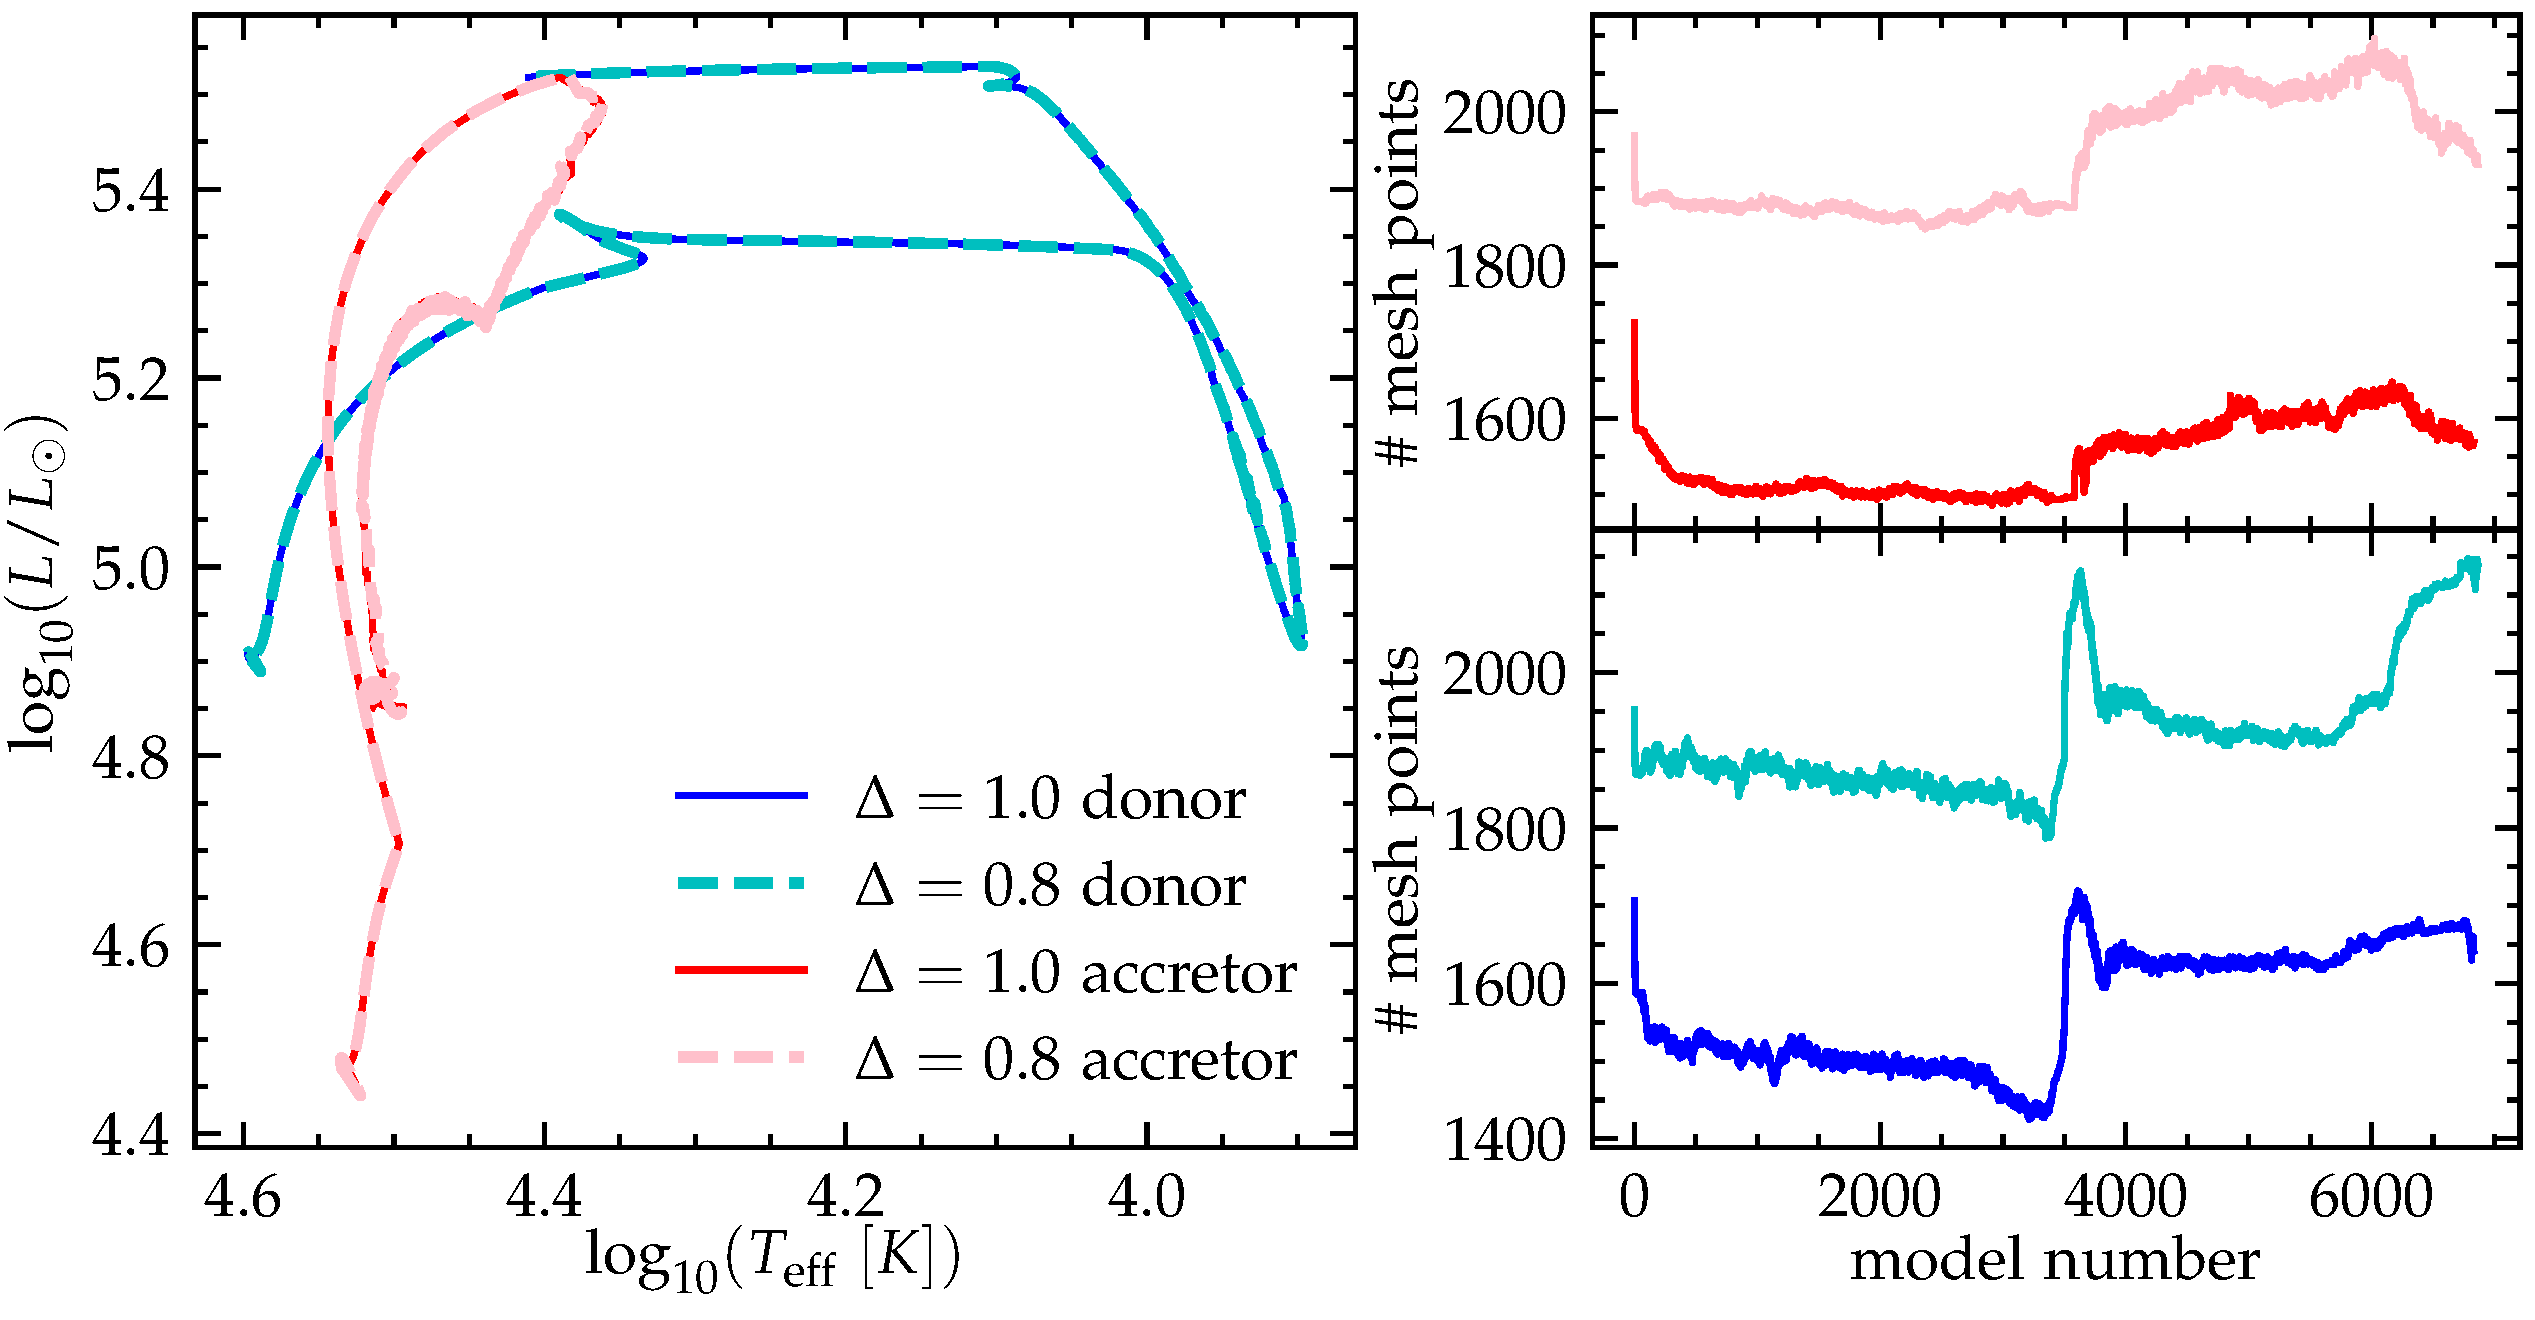
\includegraphics[width=\textwidth]{spatial_res_plot}
  \caption{Left: HRD comparison for our fiducial binary model varying
  the number of mesh points. We only show the evolution until our definition
  of RLOF detachment. Right: number of mesh points as a
  function of timestep number. In both panels, the blue/cyan tracks show the donor stars, the
red/pink tracks show the accretor. Thicker dashed lines correspond to
the models at higher resolution (i.e., lower $\Delta$ which indicates
the value of \texttt{mesh\_delta\_coeff}).}
\end{figure*}


\bibliographystyle{aasjournal}
\bibliography{./zeta_ophiuchi.bib}

\end{document}

%%% Local Variables:
%%% mode: latex
%%% TeX-master: t
%%% End:
